\documentclass{beamer}

\usetheme{default}
\title{A Distribution For Magnetic Fields}
\author{Federico Zertuche, CENBIO, UTE}
\date{\today}

\begin{document}

\begin{frame}
\titlepage
\end{frame}

\begin{frame}{A Distribution For Magnetic Fields}
The team:
\begin{itemize}
  \item[] Diego Ortiz, UNIR (Math).
  \item[] Me, UTE (Applied Math).
  \item[] Wladimir Banda, Hamburg University (Physics).
\end{itemize}
\end{frame}


\begin{frame}{A Distribution For Magnetic Fields}
 \textbf{What we study:}
 \begin{itemize}
  \setlength\itemsep{1em}
  \item[] Role of galactic winds and outflows in galaxy evolution.
  \item[] Remove gas and metals from the disk and nuclear regions of star-forming galaxies and deposit them in the circumgalactic medium.
\end{itemize}
\end{frame}


\begin{frame}{A Distribution For Magnetic Fields}
  \textbf{What we want to understand:}
\begin{itemize}
  \setlength\itemsep{1em}
  \item[] The presence of cold gas (clouds) in such outflows.
\end{itemize}


\textbf{The Wind/Shock - Cloud simulations:}
\begin{itemize}
  \item[] Transport via momentum transfer from hot gas?
  \begin{itemize}
    \item[$\cdot$] In purely hydrodynamic regimes: Too many instabilities, cloud gets destroyed rapidly.
    \item[$\cdot$] Recent simulations show that magnetic stresses can aid cloud acceleration and survival.
  \end{itemize}
\end{itemize}
\end{frame}

\begin{frame}{A Distribution For Magnetic Fields}

  \textbf{In this talk:}
  \begin{itemize}
    \setlength\itemsep{1em}
    \item[$\cdot$] Tools for a systematic statistical study of the effect of magnetic fields.
  \end{itemize}

  \vspace{1em}
  \textbf{Need: Probaility distribution over magnetic fileds.}

  (Herr W.: For magnetic fields with compact support, sometimes symmetric and div-free! And... depending on the day turbelent too.)

\end{frame}


\begin{frame}{A Distribution For Magnetic Fields}
  \textbf{Need: Probaility distribution over $f: \mathbf{R}^m \rightarrow \mathbf{R}^n$.}

  \textbf{Gaussian Process:} A proba. distribution over a function space.

  \begin{equation*}
    f(x) \sim \mathbf{GP}\left( 0,\ k(x, x')\right)
  \end{equation*}

  For any $\mathbf{x} := [x_1, ... , x_n]^T$,

  \begin{equation*}
    f(\mathbf{x}) \sim
    \mathbf{N}
    \left(
    \begin{bmatrix} 0 \\ \vdots \\ 0 \end{bmatrix},
    \begin{bmatrix}
      k(x_1, x_1) \cdots  k(x_1, x_n)\\
      \ddots \\
      k(x_n, x_1) \cdots  k(x_n, x_n)
    \end{bmatrix}
    \right)
  \end{equation*}

  where $f(\mathbf{x}) := [f(x_1), ... , f(x_n)]^T$.

\end{frame}

\begin{frame}{A Distribution For Magnetic Fields}

  \textbf{Which function space?} You get choose by chossing the covariance function $k$.

  \begin{figure}
    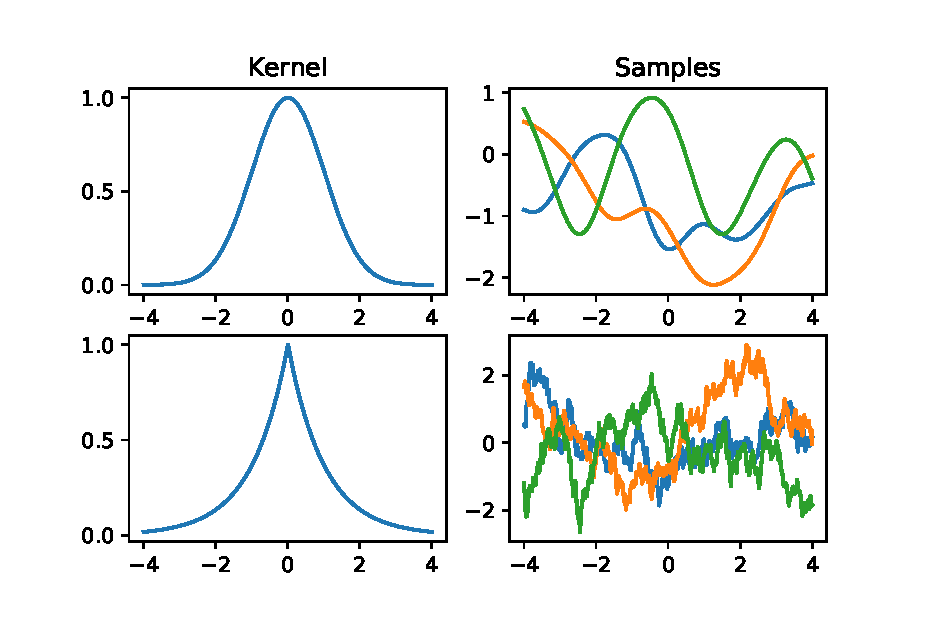
\includegraphics[width=\linewidth]{plots/regularity.eps}
  \end{figure}

\end{frame}

\begin{frame}{A Distribution For Magnetic Fields}

  \textbf{Algebra of Kernels} Can combine kernels to encode other characteristics: $k_1 \times k_2$

  \begin{figure}
    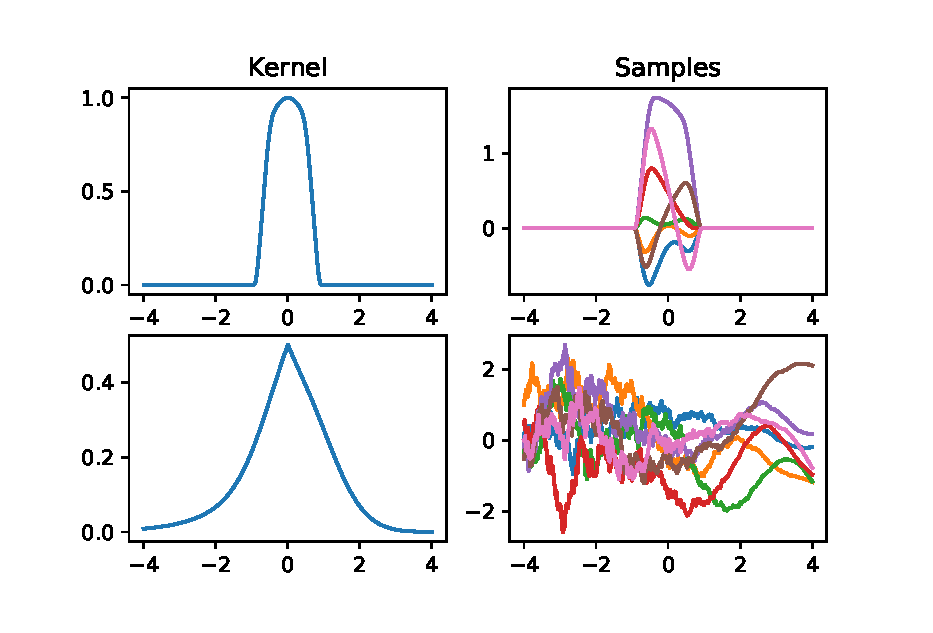
\includegraphics[width=\linewidth]{plots/multiply.eps}
  \end{figure}

\end{frame}

\begin{frame}{A Distribution For Magnetic Fields}

  \textbf{Algebra of Kernels} Can combine kernels to encode other characteristics: $k_1 + k_2$

  \begin{figure}
    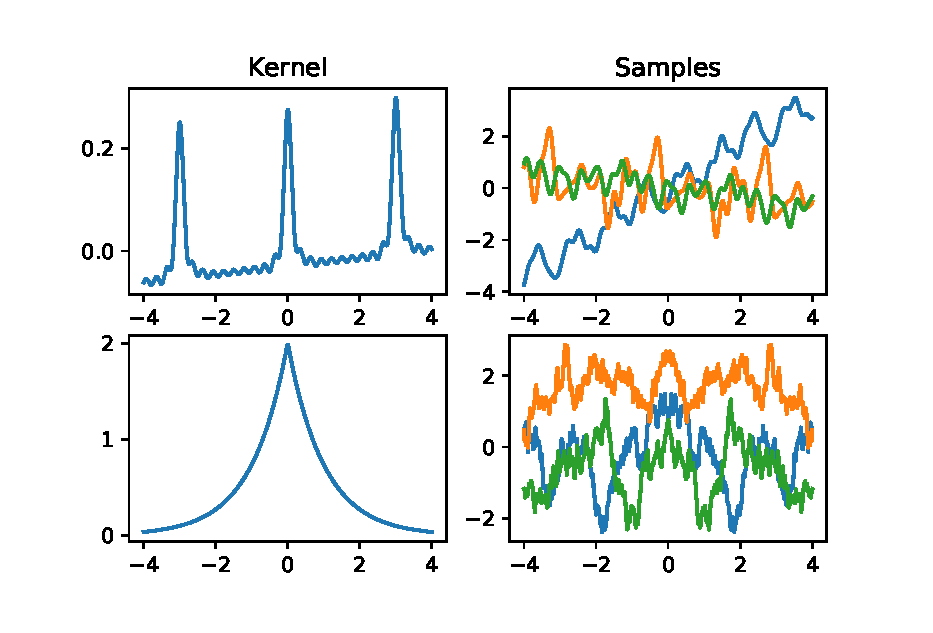
\includegraphics[width=\linewidth]{plots/sum.eps}
  \end{figure}

\end{frame}

\begin{frame}{A Distribution For Magnetic Fields}

  In fact you can encode more:

  \vspace{1em}

  \textbf{Div-Free}:

  \begin{equation*}
    \nabla f = 0
  \end{equation*}

  i.e. Processes that satisfy a linear contraint.

  \begin{equation}\label{eq:linCond}
    \mathcal{L}f = 0
  \end{equation}

  (Idea: Find an operator $\mathcal{G}$ such that $\mathcal{L}\mathcal{G} = 0$. Then, $\mathcal{G}f$ satisfies (\ref{eq:linCond}).)
\end{frame}

\begin{frame}{A Distribution For Magnetic Fields}

  \textbf{Div-Free}: Samples from a div-free \textbf{GP}.

  \begin{figure}
    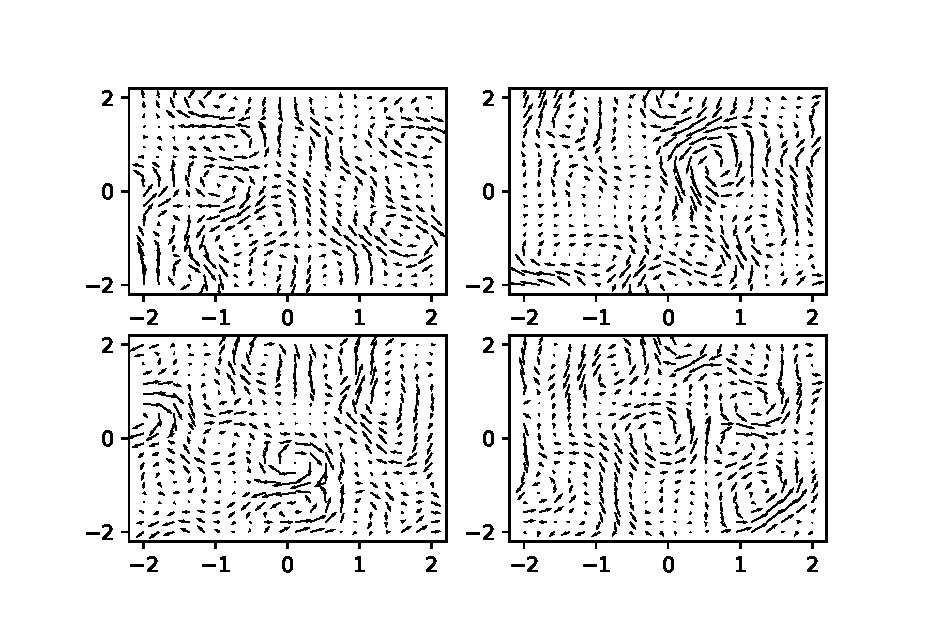
\includegraphics[width=\linewidth]{plots/div_free.eps}
  \end{figure}

\end{frame}

\begin{frame}{A Distribution For Magnetic Fields}

  \textbf{Curl-Free}: Samples from a curl-free \textbf{GP}.

  \begin{figure}
    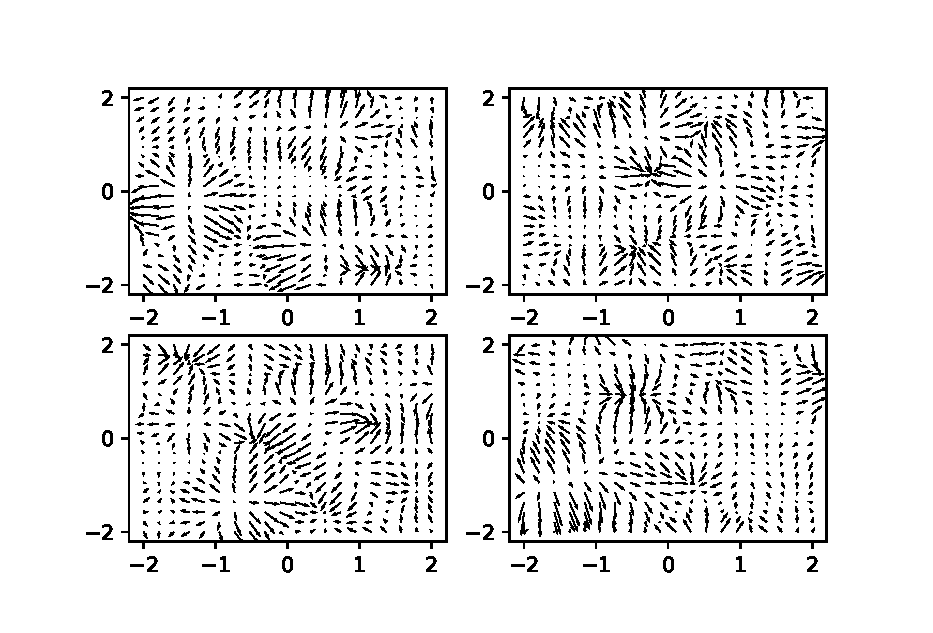
\includegraphics[width=\linewidth]{plots/curl_free.eps}
  \end{figure}

\end{frame}

\end{document}
